\documentclass{beamer}
\usetheme{Boadilla}
\usecolortheme{whale}
\usepackage{comment}
\usepackage{ragged2e}
\usepackage{amsmath}
\usepackage{dcolumn}
\usepackage{booktabs}
\usepackage{pdflscape}
\usepackage{graphicx}
\usepackage{placeins}
\usepackage{dcolumn}
\usepackage{xcolor}
\usepackage{booktabs}
\linespread{1.5}
\usepackage{subcaption}
\usepackage{amsmath}
\usepackage{hyperref}
\usepackage{multirow}
\usepackage{tikz}
\usepackage[title]{appendix}
\usetikzlibrary{decorations.pathreplacing}
\usepackage{booktabs}
\usepackage{tabularx}
%\usepackage{xepersian}
%\settextfont{XB Zar}
%\setdigitfont{XB Zar}


\renewcommand{\today}{\ifcase \month \or January\or February\or March\or %
April\or May \or June\or July\or August\or September\or October\or November\or %
December\fi, \number \year} 


\AtBeginSection[]
{
    \begin{frame}
        \frametitle{Table of Contents}
        \tableofcontents[currentsection]
    \end{frame}
}

\title[Speculative Betas]{Speculative Betas\footnote{ \tiny Jornal of Finance - 2016}}
\subtitle{Harrison Hong \qquad David A.Sraer}
\author[Aghajanzadeh]{S.M. Aghajanzadeh  }
\institute[]{Tehran Institute for Advanced Studies }
\centering

\begin{document}

{\maketitle}
\small

\section{Introduction}

\begin{frame}{Asset pricing theory}
\begin{itemize}
\item Higher beta , higher expexted return
\begin{enumerate}
\footnotesize
\item Aim to maximize economic utilities.
\item Are rational and risk-averse.
\item Are broadly diversified across a range of investments.
\item Are price takers, i.e., they cannot influence prices.
\item Can lend and borrow unlimited amounts under the risk free rate of interest.
\item Trade without transaction or taxation costs.
Deal with securities that are all highly divisible into small parcels.
\item Assume all information is available at the same time to all investors.
\end{enumerate}

\end{itemize}
\end{frame}

\begin{frame}{High-risk, low-return puzzle}
\begin{itemize}
\item Black (1972)  by relaxing the assumption of borrowing at the risk-free rate or noise traders  in Delong et al. (1990) or liquidity shocks as in Campbell, Grossman, and Wang (1993)  reconcile a flat Security Market Line
\item   We show that by relaxing the other CAPM assumptions of
\begin{enumerate}
\item  homogeneous expectations
\item costless short-selling
\end{enumerate}  can deliver rich patterns in the Security Market Line, including an inverted-U shape or even a downward-sloping line
\end{itemize}
\end{frame}


\begin{frame}{Main Results}
\begin{itemize}
\item High-beta assets are overpriced compared to low beta assets when disagreement is high:
\begin{itemize}
\tiny
\item beta amplifies disagreement about the macroeconomy. 
Because of short-sales constraints, high-beta stocks are only held in equilibrium by optimists, as pessimists are sidelined.
\end{itemize}
\item Testable implications:
\begin{itemize}
\tiny
\item Macrodisagreement is low, all investors are long and short-sales constraints do not bind
\item  For high enough aggregate disagreement, the
relationship between risk and return takes on an inverted-U shape
\end{itemize}
\item Stocks’ cash flow process is heteroskedasticity
\begin{itemize}
\tiny
\item 	large idiosyncratic variance makes optimist investors reluctant to demand of a stock
\end{itemize}
\end{itemize}
\end{frame}

\section{Model}

\begin{frame}{Model}{Assets}
\begin{itemize}
\item $ \forall i \in \{1,\dots, N\}, \tilde{d}_i = d + b_i \tilde{z} + \tilde{\epsilon}_i $ 
\begin{itemize}
\footnotesize
\item $ E[\tilde{z}] = 0 , Var[\tilde{z}] = \sigma ^2_z$
\item  $ E[\tilde{\epsilon}_i] = 0 , Var[\tilde{\epsilon}_i] = \sigma ^2_{\epsilon}$  
\end{itemize}
\item $ s_i = \frac{1}{N} $
\item $ 0<b_1 <b_2<\dots<b_N $
\end{itemize}
\end{frame}

\begin{frame}{Invesots}
\begin{itemize}
\item Heterogeneous investors (fractio $ \alpha $) 
\begin{itemize}
\item Cannot short
\item Two groups:
\begin{itemize}
\item A : $ E^A[\tilde{z}] = \lambda $
\item B : $ E^B[\tilde{z}] = -\lambda $
\end{itemize}
\end{itemize}
\item Homogeneous investors (fractio $ 1-\alpha $) 
\begin{itemize}
\item No short-sales constraint
\item $ E^a[\tilde{z}] = 0 $
\end{itemize}
\item Investor's utility:
\begin{equation*}
U(\tilde{w}^k) = E^k[\tilde{w}^k] - \frac{1}{2\gamma}Var(\tilde{w}^k) \text{\qquad} k\in\{a,A,B\}
\end{equation*}
\end{itemize}
\end{frame}


\begin{frame}{Equilibrium}
\begin{itemize}
\item Asset prices:
\begin{equation*}
P_i(1+r) = \left\{\begin{array}{ll}
d - \frac{1}{\gamma}(b_i\sigma^2_z+\frac{\sigma^2_{\epsilon}}{N}) & \text{ for } i< \bar{i}\\
d - \frac{1}{\gamma}(b_i\sigma^2_z+\frac{\sigma^2_{\epsilon}}{N}) + \underbrace{\frac{\theta}{\gamma}(b_i\sigma^2_z\omega(\lambda)-\frac{\sigma^2_{\epsilon}}{N})}_{\pi^i = \text{speculative premimum}} & \text{ for } i \geq \bar{i} 
\end{array}
\right.
\end{equation*}
$\footnotesize \omega(\lambda) = \frac{\lambda\gamma - \frac{\sigma^2_z}{N}(\sum_{i\geq\bar{i}}b_i)}{\sigma^2_z(1+\sigma^2_z(\sum_{i<\bar{i}}\frac{b^2_i}{\sigma^2_{\epsilon}}))} $ \qquad $\scriptsize \theta = \frac{\frac{\alpha}{2}}{1-\frac{\alpha}{2}} $
\item If $ \alpha = 0 $ then $ \theta = 0 $ , As a result $ \pi^i = \text{speculative premimum} $
\item $\lambda  \uparrow \pi^i \uparrow $ \qquad $b_i  \uparrow \pi^i \uparrow $  \qquad $\alpha  \uparrow \pi^i \uparrow $ 
\end{itemize}
\end{frame}

\begin{frame}{Equilibrium}{Beta and Expected Return}
\begin{itemize}
\item Expected excess return :
\begin{equation*}
E[\tilde{R}_i^e] = \left\{\begin{array}{ll}
\beta_i\frac{\sigma^2_z+\frac{\sigma^2_{\epsilon}}{N}}{\gamma}& \text{ for } i< \bar{i}\\
\beta_i\frac{\sigma^2_z+\frac{\sigma^2_{\epsilon}}{N}}{\gamma}(1-\theta\omega(\lambda)) + \theta  \frac{\sigma^2_{\epsilon}}{\gamma N}(1+\omega(\lambda))& \text{ for } i \geq \bar{i}
\end{array}
\right.
\end{equation*}
\item Expected excess return (Heteroskedastic Idiosyncratic Variance) :
\begin{equation*}
E[\tilde{R}_i^e] = \left\{\begin{array}{ll}
\beta_i\frac{\sigma^2_z+\sum_{j=1}^{N}\frac{\sigma^2_{j}}{N}}{\gamma}& \text{ for } \frac{\beta_i}{\sigma^2_i} < \frac{\beta_{\bar{i}}}{\sigma^2_{\bar{i}}}\\
\beta_i\frac{\sigma^2_z+\sum_{j=1}^{N}\frac{\sigma^2_{j}}{N}}{\gamma}(1-\theta\omega(\lambda)) + \theta  \frac{\sigma^2_{i}}{\gamma N}(1+\omega(\lambda))& \text{for} \frac{\beta_i}{\sigma^2_i} \geq \frac{\beta_{\bar{i}}}{\sigma^2_{\bar{i}}}
\end{array}
\right.
\end{equation*}
\end{itemize}
\hfill\hyperlink{Proof}{\beamerbutton{Proof}}
\end{frame}

\begin{frame}{Security Market Line}{different levels of aggregate disagreement}
\begin{figure}
\centering
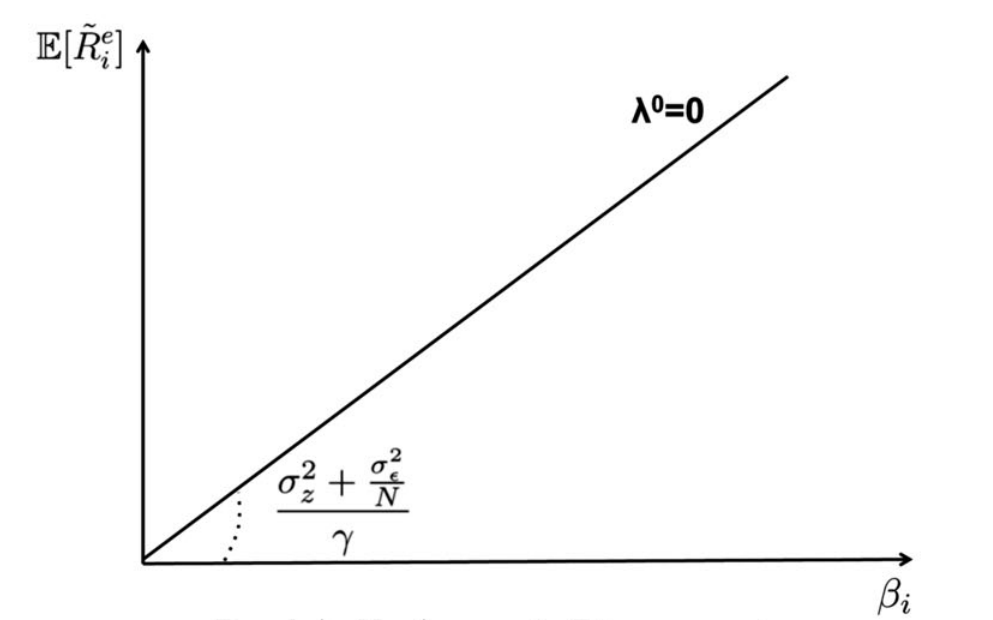
\includegraphics[width=0.32\linewidth]{1}
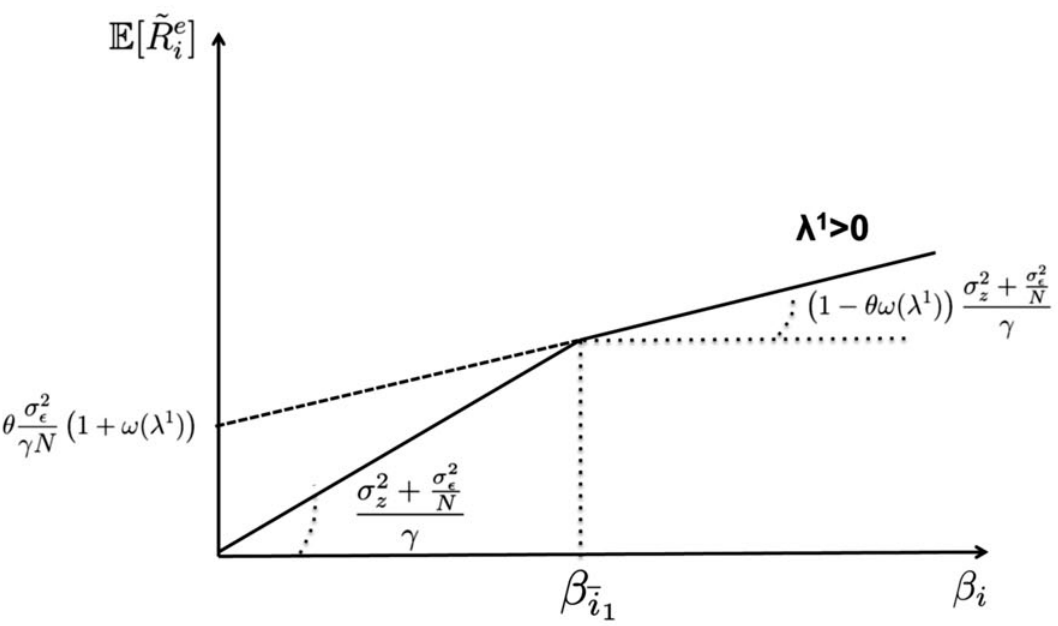
\includegraphics[width=0.32\linewidth]{2}
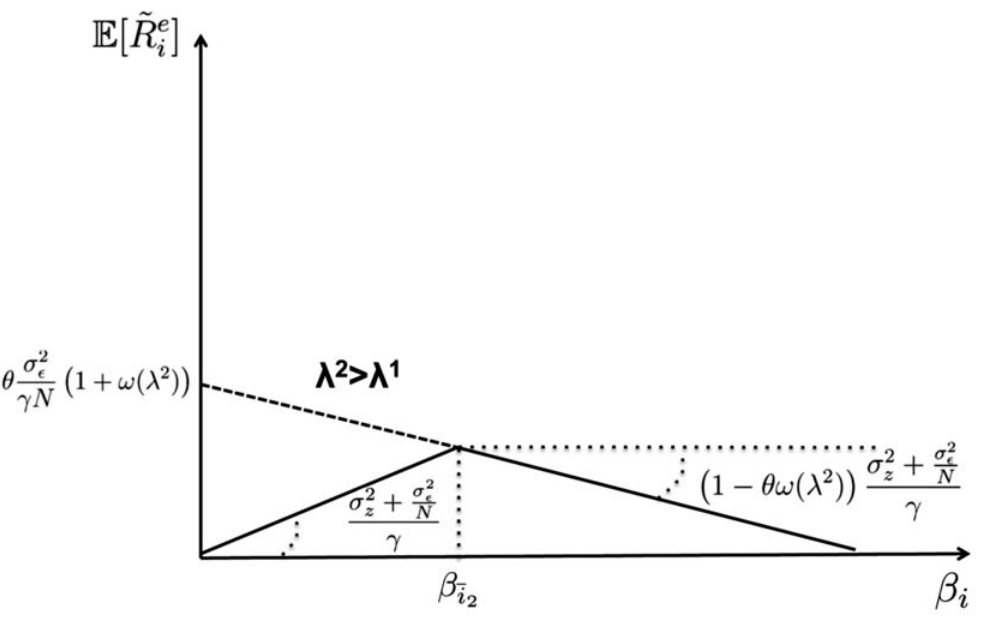
\includegraphics[width=0.32\linewidth]{3}
\label{fig:indimb}
\end{figure}
\end{frame}
\section{Emperical Works}
\begin{frame}{$ \beta $-Sorted Portfolios}
\begin{itemize}
\item At the beginning of each calendar month, stocks are ranked in ascending order on the basis of their estimated beta at the end of the previous month
\item The ranked stocks are assigned to 1 of 20 value-weighted portfolios
\end{itemize}
\begin{figure}
\centering
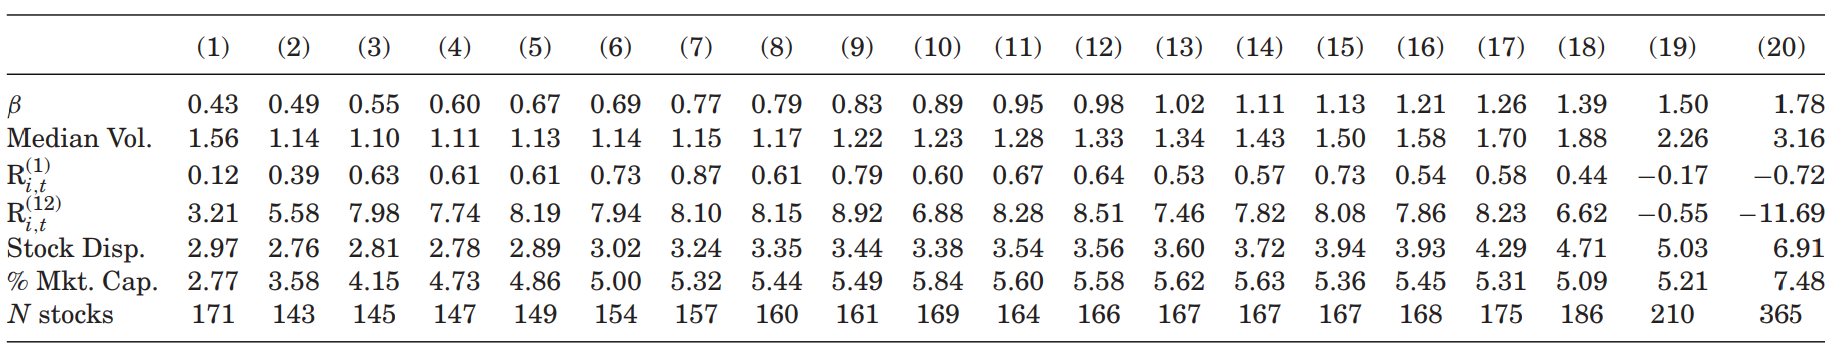
\includegraphics[width=0.9\linewidth]{t1}
\end{figure}
\end{frame}

\begin{frame}{Measuring Aggregate Disagreement}
\begin{itemize}
\item Measure stock-level disagreement as the dispersion in analyst forecasts
\item Aggregate this stock-level disagreement measure,
weighting each stock by its preranking $ \beta $ 
\end{itemize}
\begin{figure}
\centering
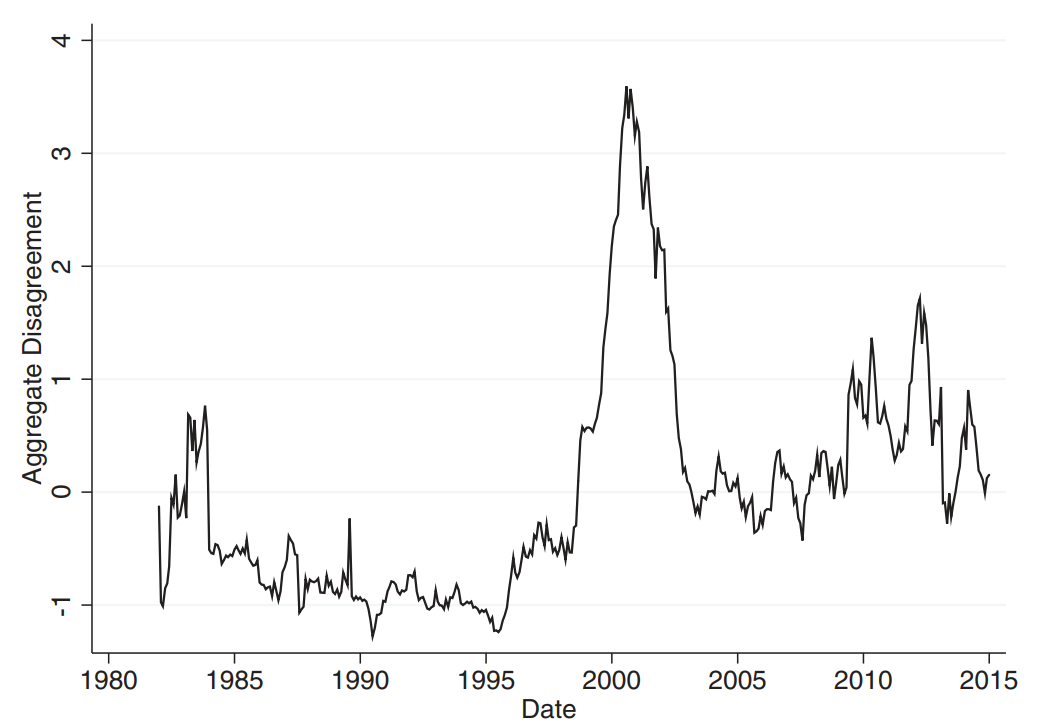
\includegraphics[width=0.45\linewidth]{4}
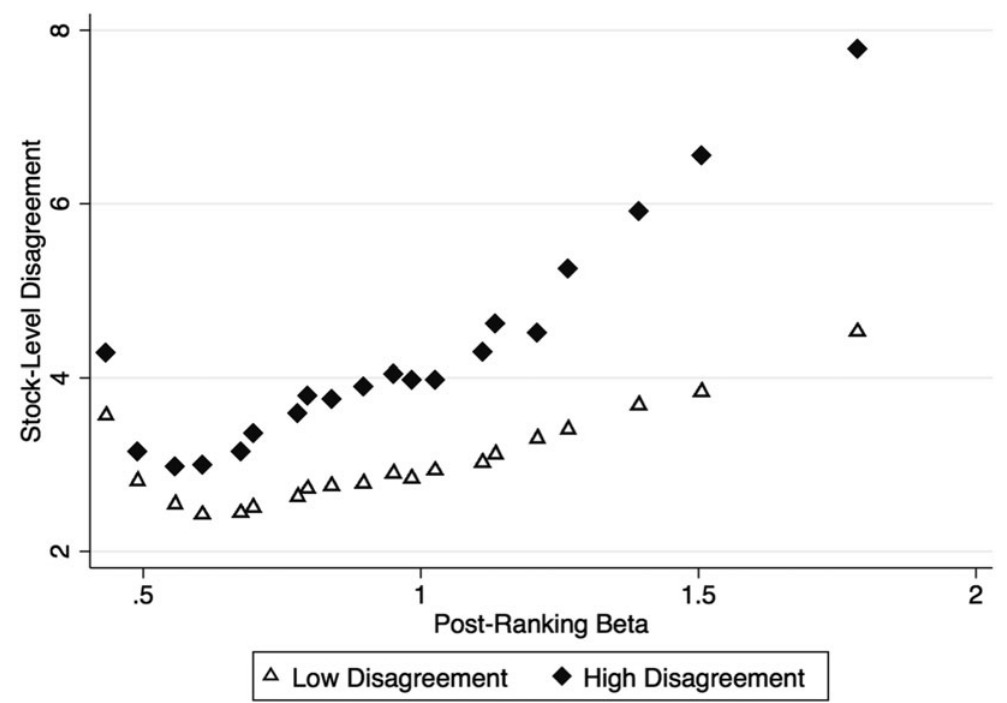
\includegraphics[width=0.45\linewidth]{5}
\end{figure}
\end{frame}

\begin{frame}{Concavity of the Security Market Line}
\begin{itemize}
\item  Average excess returns-to-$ \beta $ relationship is mostly
upward-sloping 
\item   Inverted-U shape predicted by the theory
\end{itemize}
\begin{figure}
\centering
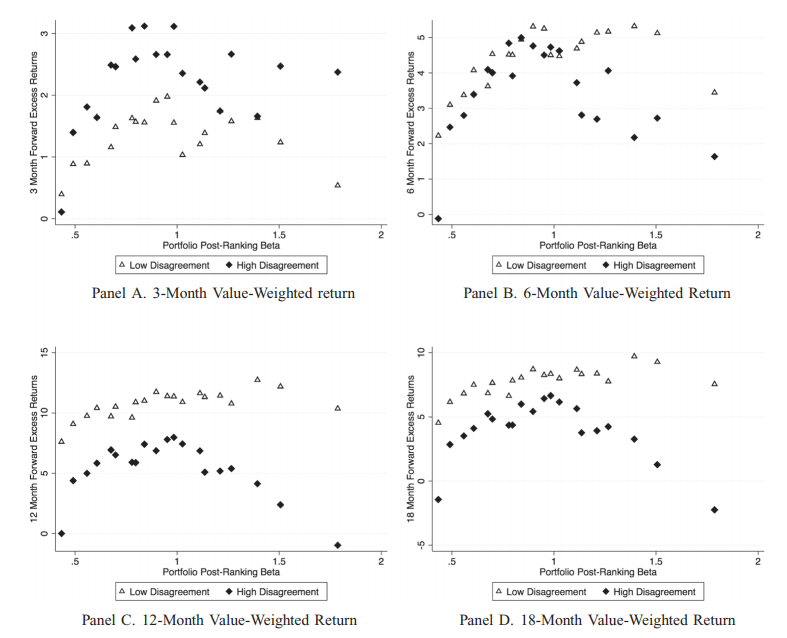
\includegraphics[width=0.5\linewidth]{6}
\end{figure}
\end{frame}

\begin{frame}{Formally test}
\begin{itemize}
\item two-stage Fama and MacBeth regression

\item First Stage: \begin{equation*}
r_{P,t}^{(12)} = \kappa_t + \pi_t \times \beta_P + \phi_t \times (\beta_P)^2 + \epsilon_{P,t}
\end{equation*}
\item Second Stage:
\begin{equation*}
\tiny
\left\{\begin{array}{l}
 \phi_t  = c_1 + \psi_1 . Dis_{t-1} + \delta^m_1 . R^{(12)}_{m,t} + \delta^{HML}_1. HML^{(12)}_t + \delta^{SMB}_1. SMB^{(12)}_t  + \delta^{UMD}_1. UMD^{(12)}_t + \sum_{x\in X}\delta^x_1.x_{t-1} + \zeta_t \\\\
  \pi_t  = c_2 + \psi_2 . Dis_{t-1} + \delta^m_2 . R^{(12)}_{m,t} + \delta^{HML}_2. HML^{(12)}_t + \delta^{SMB}_2. SMB^{(12)}_t  + \delta^{UMD}_2. UMD^{(12)}_t + \sum_{x\in X}\delta^x_2.x_{t-1} + \zeta_t 
  \\\\
    \kappa_t  = c_3 + \psi_3 . Dis_{t-1} + \delta^m_2 . R^{(12)}_{m,t} + \delta^{HML}_3. HML^{(12)}_t + \delta^{SMB}_3. SMB^{(12)}_t  + \delta^{UMD}_3. UMD^{(12)}_t + \sum_{x\in X}\delta^x_2.x_{t-1} + \zeta_t 
\end{array}\right.
\end{equation*}

\end{itemize}
\end{frame}

\begin{frame}{Estimation ressults}
\begin{figure}
\centering
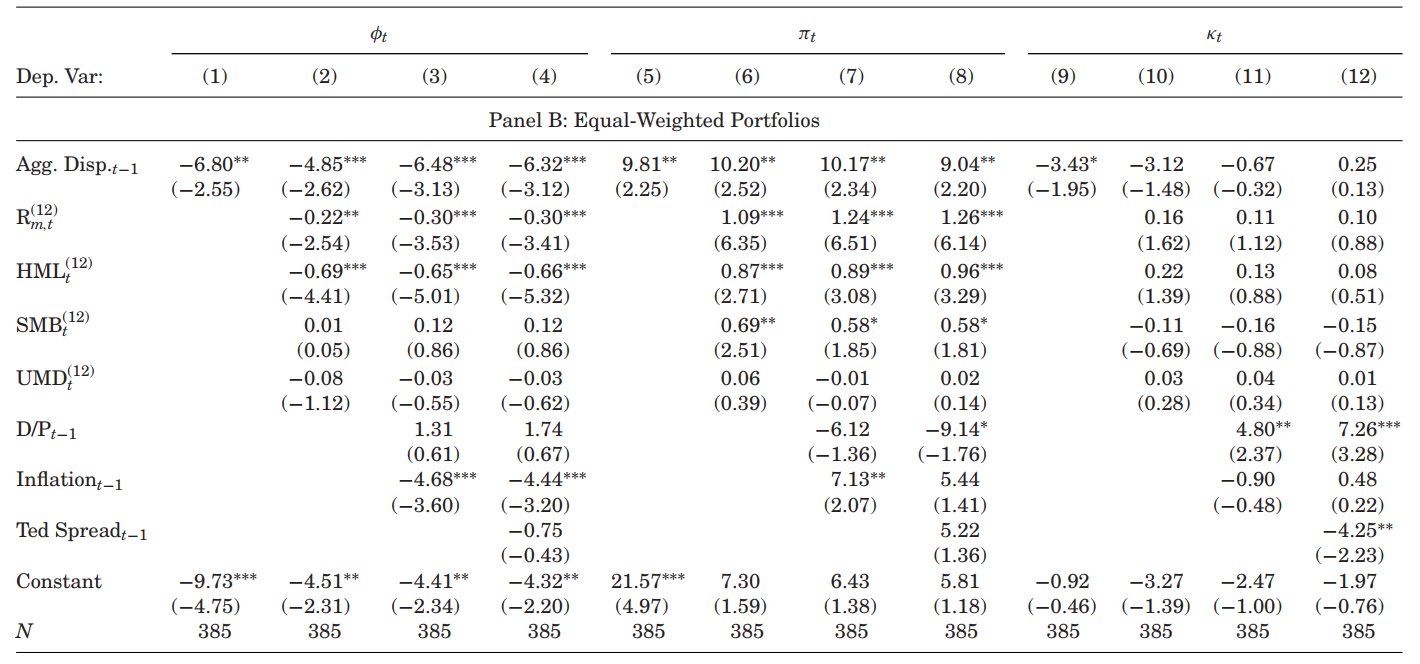
\includegraphics[width=0.85\linewidth]{t2}
\end{figure}
\end{frame}



\begin{frame}{$ \beta $-Sorted Portfolios}
\begin{itemize}
\item Rank stocks based on preranking ratio of $ \beta $ to $ \sigma^2 $ and define as speculative stocks all stocks with a ratio above  the  median ratio
\item Then, within each of these two groups creat 20 $ \beta $-sorted portfolios
\end{itemize}
\begin{figure}
\centering
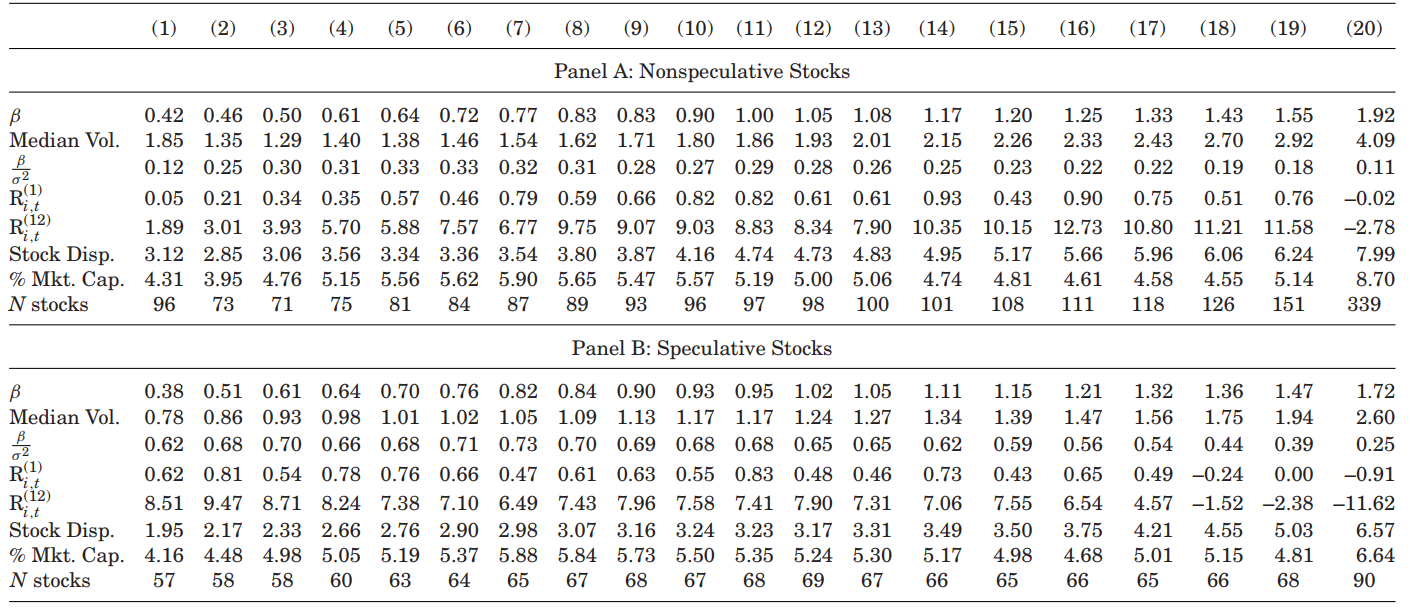
\includegraphics[width=0.8\linewidth]{t3}
\end{figure}
\end{frame}




\begin{frame}{Concavity of the Security Market Line}
\begin{itemize}
\tiny
\item For nonspeculative stocks, the Security Market Line is not related with aggregate disagreement. 
\item For speculative stocks when aggregate disagreement is high, the Security Market Line exhibits an inverted-U shape
\end{itemize}
\begin{figure}
\begin{subfigure}[t]{.45\linewidth}
    \centering
    \tiny
    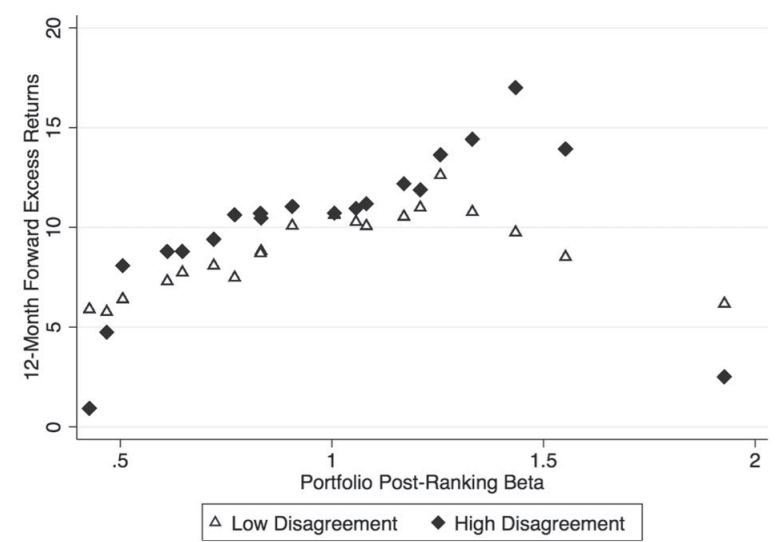
\includegraphics[width=1\linewidth]{7}
    \caption{Nonspeculative Stocks}
  \end{subfigure}
  \begin{subfigure}[t]{.45\linewidth}
    \centering
    \tiny
    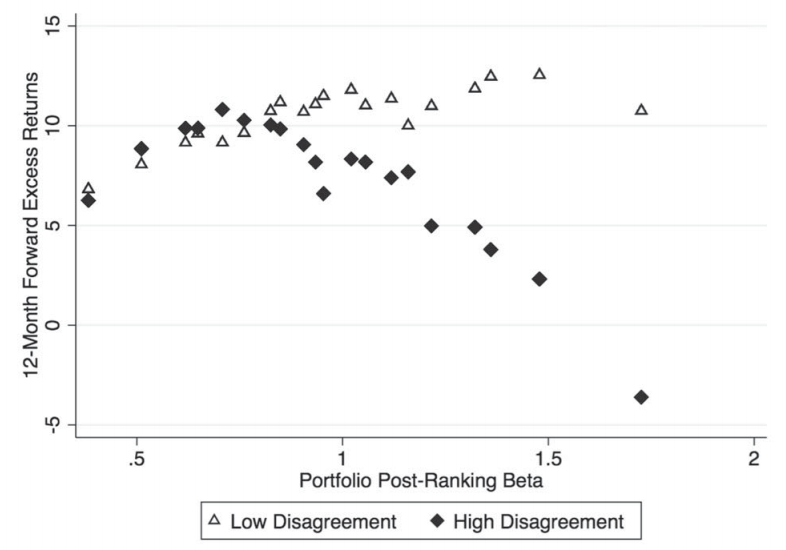
\includegraphics[width=1\linewidth]{8}
    \caption{Speculative Stocks}
  \end{subfigure}
\end{figure}
\end{frame}

\section{Conclusion}
\begin{frame}{Conclusion}
\begin{itemize}
\item High-beta assets are more speculative because they are more sensitive to disagreement about common cash flows
\item As aggregate disagreement rises, the slope of the Security Market Line is piecewise constant, higher in the low-beta range and potentially negative for the highbeta range
\end{itemize}
\end{frame}
\appendix
\section{Iran's Data}

\begin{frame}{Return \& $ \beta $}

\begin{figure}
\centering
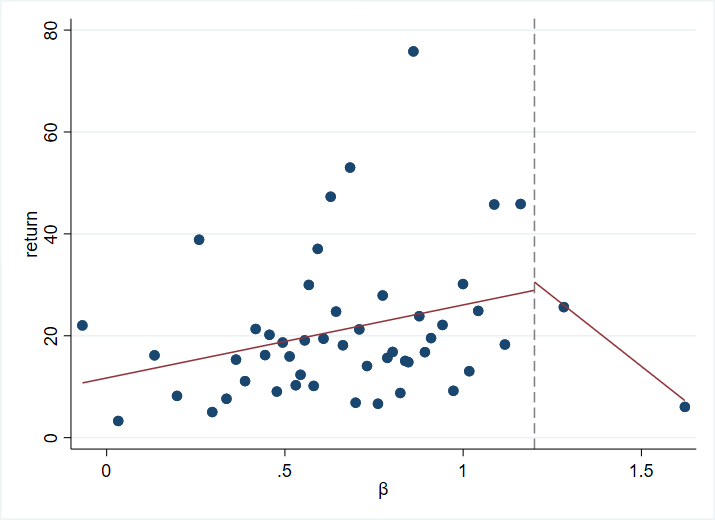
\includegraphics[width=0.45\linewidth]{mygraph1}
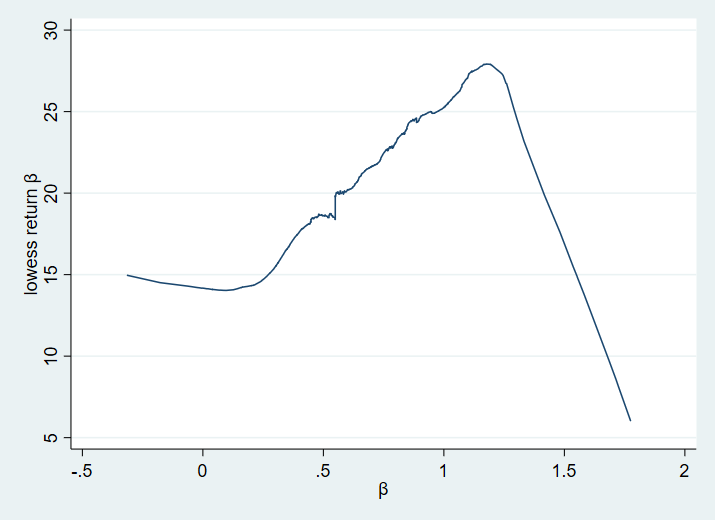
\includegraphics[width=0.45\linewidth]{mygraph2}
\label{fig:mygraph0}
\end{figure}

\end{frame}

\begin{frame}{Return \& $ \beta/\sigma $}
\begin{figure}
\centering
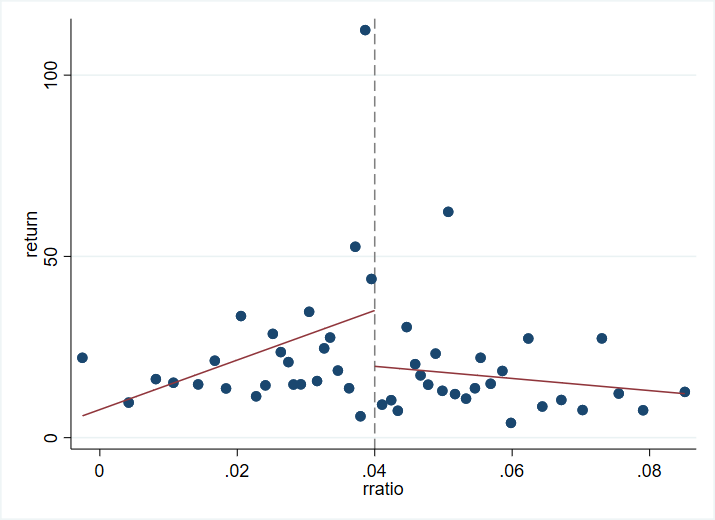
\includegraphics[width=0.45\linewidth]{mygraph3}
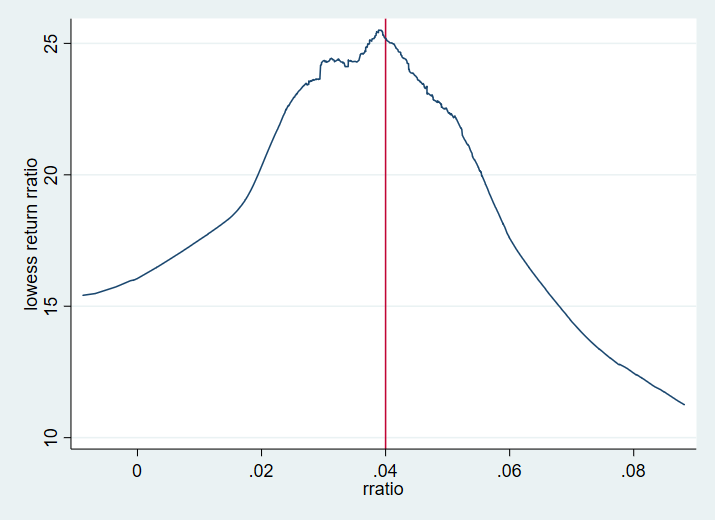
\includegraphics[width=0.45\linewidth]{mygraph4}

\label{fig:mygraph4}
\end{figure}
\end{frame}



\section{Proof}
\begin{frame}{Equilibrium}{Beta and Expected Return}
\label{Proof}
\begin{itemize}
\item $\tilde{R}_i^e = d + b_i\tilde{z} + \tilde{\epsilon}_i - (1+r)P_i$
\item $ \beta_i = \frac{Cov(\tilde{R}_i^e ,\tilde{R}_m^e )}{Var(\tilde{R}_m^e)} = \frac{b_i\sigma^2_z+\frac{\sigma^2_{\epsilon}}{N}}{\sigma^2_z+\frac{\sigma^2_{\epsilon}}{N}} $
\item $ E[\tilde{R}_i^e] = d - (1+r)P_i  \rightarrow(1+r)P_i = d - E[\tilde{R}_i^e] $
\item $ d - E[\tilde{R}_i^e]  = d - \frac{1}{\gamma}(b_i\sigma^2_z+\frac{\sigma^2_{\epsilon}}{N}) + {\frac{\theta}{\gamma}(b_i\sigma^2_z\omega(\lambda)-\frac{\sigma^2_{\epsilon}}{N})} $
\item $  E[\tilde{R}_i^e] = \frac{1}{\gamma}(b_i\sigma^2_z+\frac{\sigma^2_{\epsilon}}{N}) - {\frac{\theta}{\gamma}(b_i\sigma^2_z\omega(\lambda)-\frac{\sigma^2_{\epsilon}}{N})} $
\item $  \begin{array}{ll}
E[\tilde{R}_i^e]& =    \frac{b_i\sigma^2_z+\frac{\sigma^2_{\epsilon}}{N}}{\gamma} (1-\theta\omega(\lambda)) + \theta  \frac{\sigma^2_{\epsilon}}{\gamma N}(1+\omega(\lambda)) ‌\\ 
& =\beta_i\frac{\sigma^2_z+\frac{\sigma^2_{\epsilon}}{N}}{\gamma}(1-\theta\omega(\lambda)) + \theta  \frac{\sigma^2_{\epsilon}}{\gamma N}(1+\omega(\lambda))
\end{array} $
\end{itemize}
\end{frame}

\end{document}